\documentclass[11pt,pra,aps]{revtex4}
\usepackage[dvipdfmx]{graphicx}
\usepackage{float}
\usepackage{rotating}
\usepackage{array}
\usepackage{amsmath}
\usepackage{multirow}
\usepackage{setspace}
\usepackage{braket}
\usepackage{epstopdf}
\usepackage{moreverb}
\usepackage{wrapfig}
\usepackage{longtable}

\usepackage{color}                            

\usepackage[dvipdfmx]{hyperref}
\usepackage{pxjahyper}

\newcommand{\red}[1]{\textcolor{red}{#1}}     
\newcommand{\blue}[1]{\textcolor{blue}{#1}}

\newcommand{\boxz}[1]{\boxed{\phantom{\text{#1}}}}
\newcommand{\boxa}[1]{\boxed{\phantom{}}}

%%\renewcommand{\baselinestretch}{2.0}

\renewcommand{\thefigure}{S\arabic{figure}}
\renewcommand{\thetable}{S\arabic{table}}

\begin{document}
\title{摂動論と変分法}
\author{齋藤 雅明 \\ 量子化学研究室 \\ email: masa.saitow@chem.nagoya-u.ac.jp}

\maketitle

\noindent
{\bf 問題1.} 以下の空欄を埋めよ。

% Levine 8.1
\noindent
{\bf 1.1} Li原子の基底状態エネルギーに対して3つの変分計算が行われ、その結果-203.2 eV、-192.0 eV、-201.2 eVという結果が得られた。このことからLi原子の真の基底状態エネルギーは\boxz{-203.2 eV}よりも\boxz{低い}ことが分かる。

\noindent
{\bf 1.2} 水素原子のシュレーディンガー方程式は極座標系では、同径部分と角度部分とに分離される。エネルギーは角度方程式のみから決定され、角度部分のハミルトニアンは以下の式で与えられる。
\begin{align}
  H = -\frac{\hbar^2}{2m_e r^2}\frac{d}{dr}\left(r^2\frac{d}{dr}\right)-\frac{e^2}{4\pi\epsilon_0 r}
\end{align}
この最低エネルギー固有値$E_\text{exact}$は原子単位で\boxz{-0.5}と与えられる。試行関数としてガウス型関数
\begin{align}
  \psi_\text{trial}(\alpha;r)=N\exp\left(-\alpha r^2\right) \ (\alpha\text{は変分パラメータ})
\end{align}
を用いた場合はエネルギー$E_\text{trial}$は原子単位で\boxz{}と計算される。これは変分原理を満足しており、$E_\text{exact}$\boxz{$\leq$}$E_\text{trial}$という大小関係が成立する。

\noindent
{\bf 問題2.} 以下の問いに答えよ。

% Levine 8.4
\noindent
{\bf 2.1} 次のような長さ$l$の無限に高い一次元井戸型ポテンシャル
\begin{align}
  V(x)=\left\{
  \begin{array}{cc}
    0 & (0 \leq x \leq l) \\
    \infty & (\text{それ以外})
  \end{array}
  \right.
\end{align}
中の粒子のエネルギー計算に以下の規格化された試行関数
\begin{align}
  \psi_\text{trial}(x) = \sqrt{\frac{3}{l^3}}x
\end{align}
を用いるとき、エネルギー期待値は0となり、真のエネルギーよりも低く見積もられる。この理由を述べよ。

% McQuarrie 7.8
\noindent
{\bf 2.2} 3次元球対称調和振動子の基底状態エネルギーを考える。$\alpha$を変分パラメータとする以下の二つの試行関数を用いた場合、どちらの方がより真の解に近い結果を与えるか。理由も併せて延べよ。
\begin{align}
  \psi_\text{trial}(r)&=N\exp\left(-\alpha r\right) \\
  \psi_\text{trial}(r)&=N\exp\left(-\alpha r^2\right)
\end{align}
ここでハミルトニアン演算子は
\begin{align}
  H=-\frac{\hbar^2}{2\mu r^2}\frac{d}{dr}\left(r^2\frac{d}{dr}\right)+\frac{k}{2}r^2
\end{align}
である。

\noindent
{\bf 問題3.}
%位置–運動量の不確定性関係を含む、種々の不確定性関係は以下のRobertsonの不等式より導くことができる。\footnote{証明は例えばJ. J. サクライ著「現代の量子力学 第1版」第一章にある。}
演算子$A$及び$B$で表される二つの物理量の間に存在する不確定性関係は、次のRobertsonの不等式で与えられる。\footnote{証明は例えばJ. J. サクライ著「現代の量子力学 第1版」第一章にある。}
このとき以下の問いに答えよ。計算過程は省略しても良いが、どのように考えてそのような結果が得られたかが分かるように解答すること。

\begin{align}
  \Delta A\ \Delta B \geq \frac{1}{2}|\langle\psi|[A,B]|\psi\rangle|\label{eq:Robertson}
\end{align}

\noindent
{\bf 3.1} 式(\ref{eq:Robertson})において、$A\rightarrow x$、$B\rightarrow p$として、位置-運動量間の不確定性関係を導出せよ。

\noindent
{\bf 3.2} $x-y$面上を円運動する電子について考える(図\ref{fig:circ})。球座標系を用いると角運動量のz成分を記述する演算子は以下のように与えられる。
\begin{align}
  L_z=xP_y-yP_z=-i\hbar\frac{\partial}{\partial \phi}
\end{align}
このとき式(\ref{eq:Robertson})を用いて角運動量の垂直成分$L_z$と回転角$\phi$との間の不確定性関係を計算せよ。また角度の範囲は$0\leq \phi < 2\pi$である。

\begin{wrapfigure}{r}[10pt]{0.3\textwidth}
  \centering
  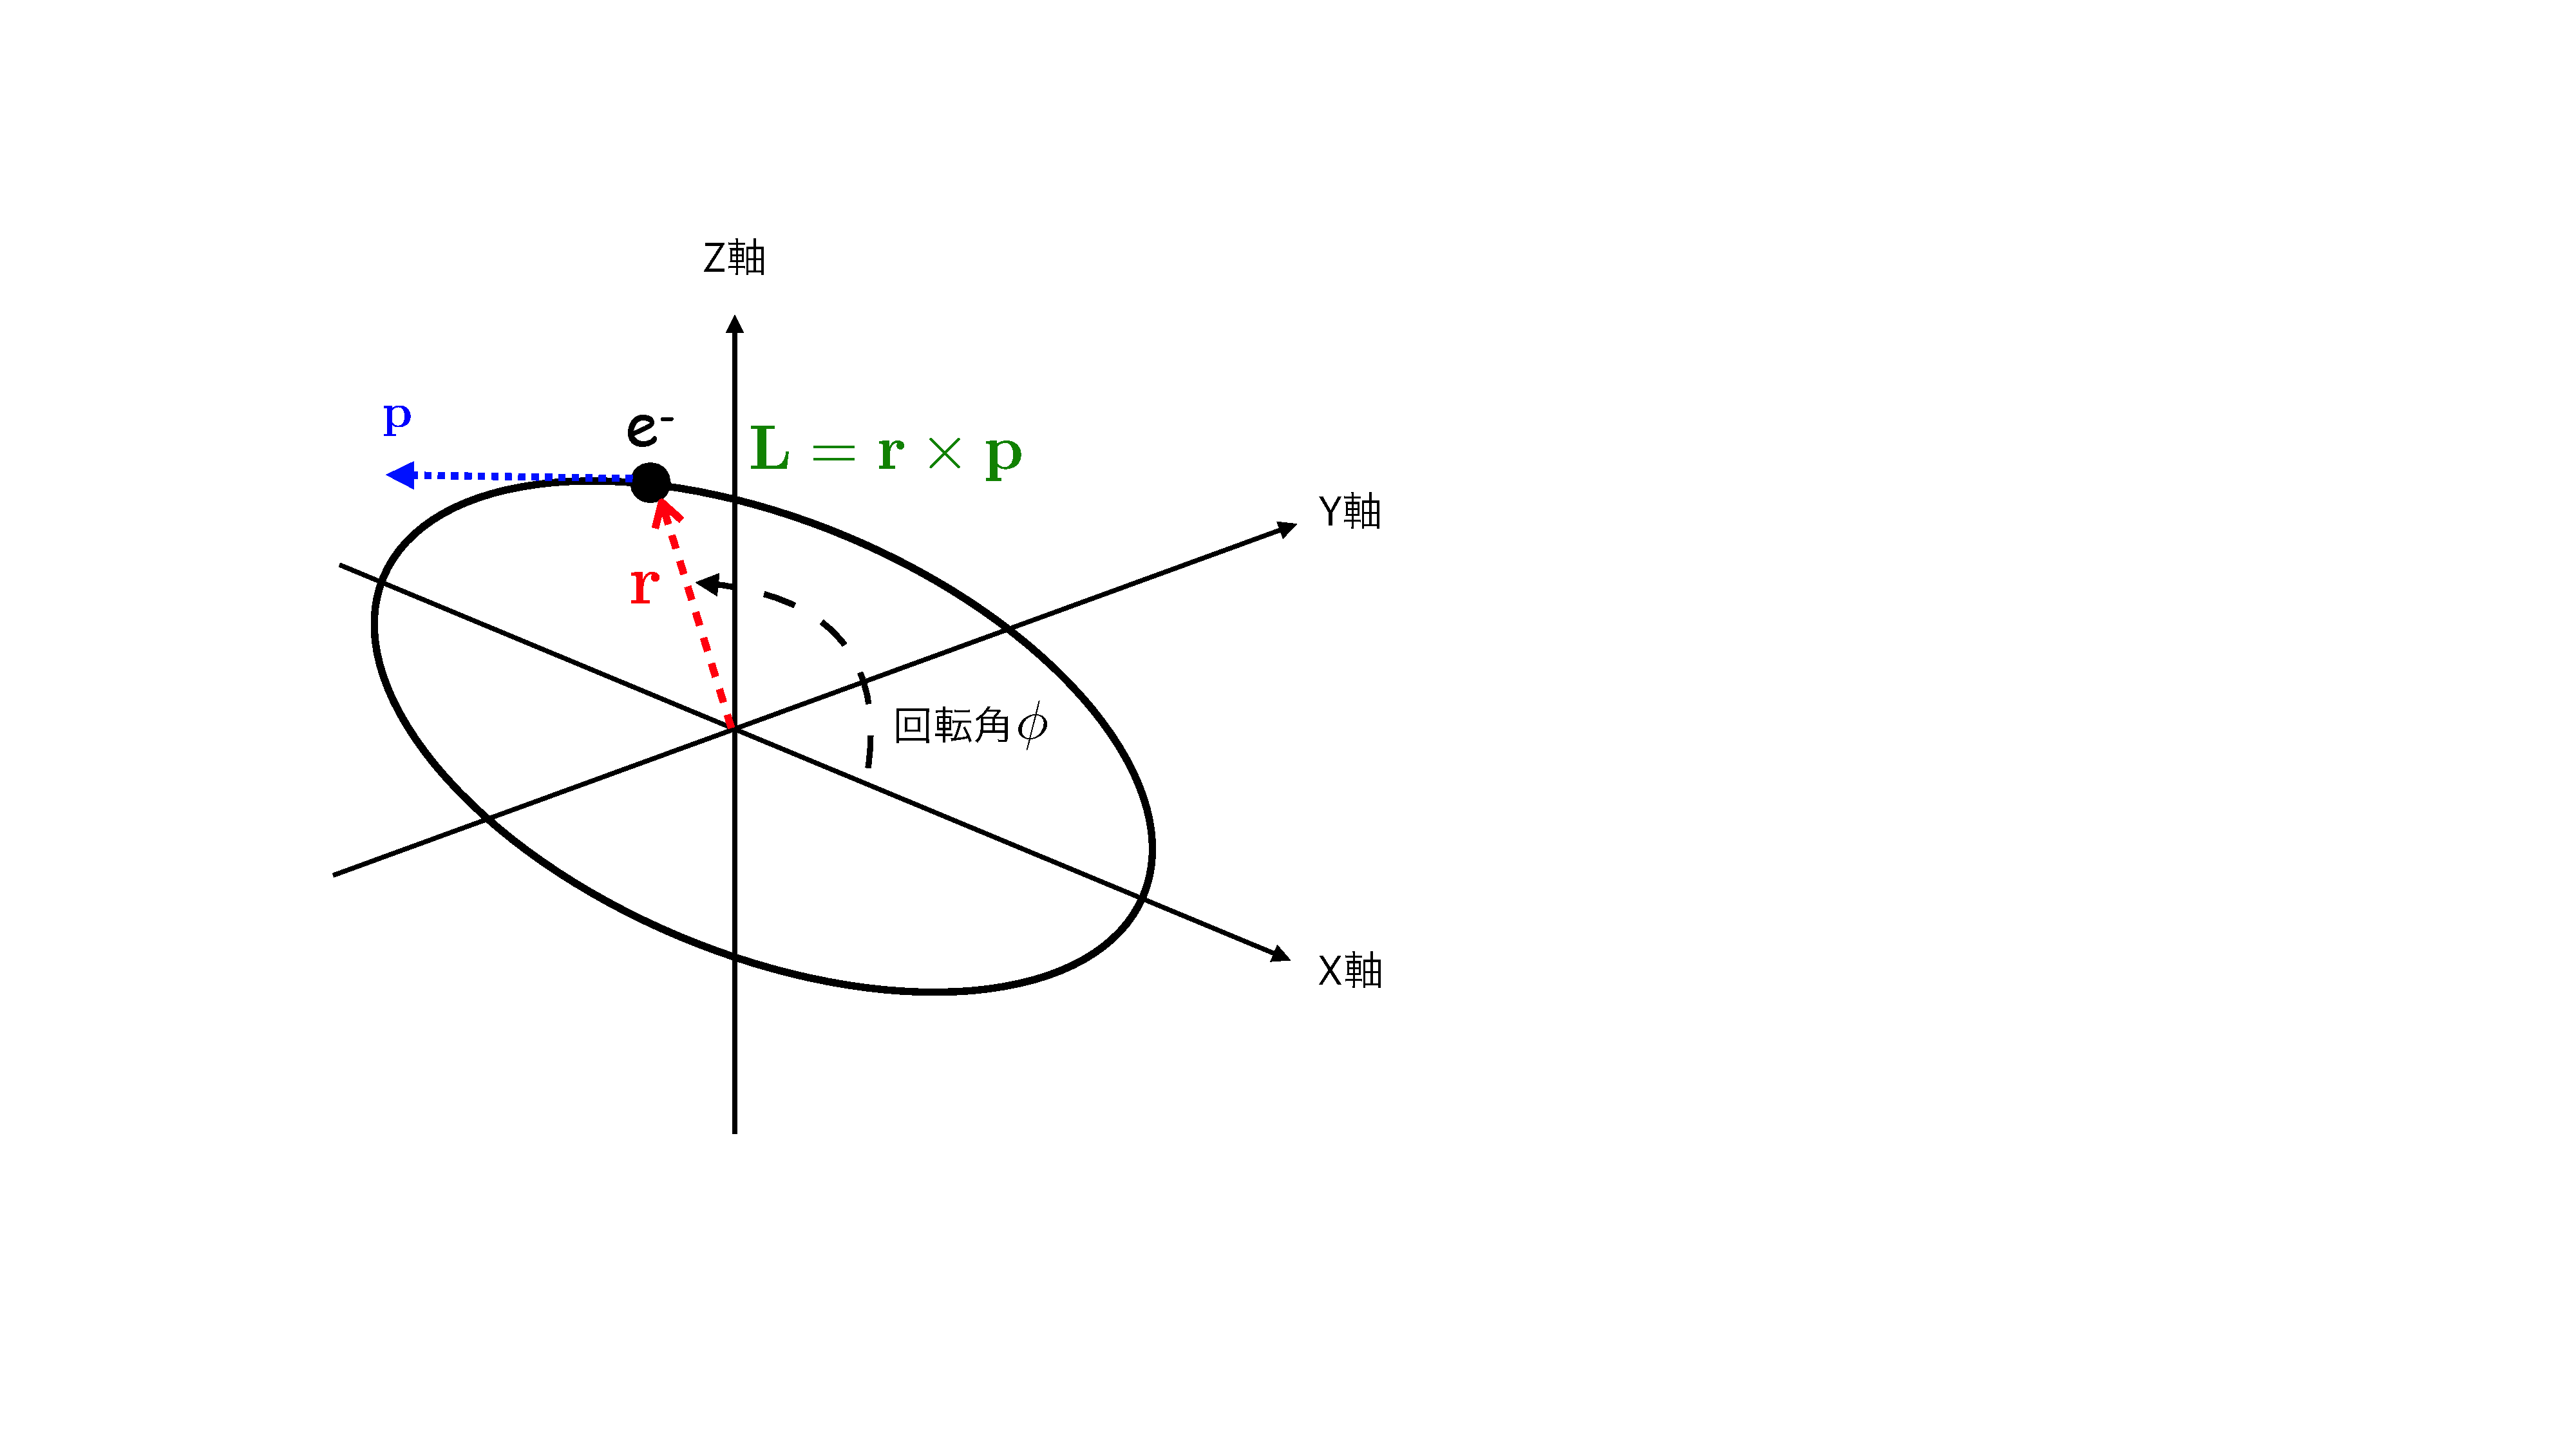
\includegraphics[width=5.5cm]{circular-motion.pdf}
  \caption{\label{fig:circ} $x-y$面上を円環運動する電子}
\end{wrapfigure}

\noindent
{\bf 3.3} 問い3.2で計算した不確定性関係はこの系に対しては正しくない。それは何故か。

\noindent
{\bf 3.4} 円環上の粒子の$L_z$と$\phi$との不確定性関係にも適用可能となるように、Krausらは式(\ref{eq:Robertson})を次のように一般化した。\footnote{K. Kraus, Z. Physik. 188, 374-377 (1965).}
\begin{align}
  \Delta A\ \Delta B \geq \frac{1}{2}\left|\int_A dx \left[(A\psi)^{*} (B\psi) - (B\psi)^{*} (A\psi)\right]\right|\label{eq:kraus}
\end{align}
ここで$A$は問題で与えられた積分範囲を意味する。式(\ref{eq:kraus})を用いて円環上の電子について$L_z$と$\phi$との不確定性関係を計算せよ。

\noindent
{\bf 問題4.} 調和振動子のSchr\"odinger方程式は以下のように与えられる。このとき以下の問いに答えよ。計算過程は省略しても良いが、どのように考えてそのような結果が得られたかが分かるように解答すること。
\begin{align}
  -\frac{\hbar^2}{2m}\frac{d^2\psi}{dx^2}+\frac{1}{2}m\omega^2x^2=E\psi \label{eq:harm}
\end{align}

\noindent
{\bf 4.1} 式(\ref{eq:harm})に以下の変換を行い、$\xi$に関する方程式を導出せよ。
\begin{align}
  \xi=ax,\ a=\sqrt{\frac{m\omega}{\hbar}},\ \epsilon=\frac{2E}{\hbar\omega}
\end{align}

\noindent
{\bf 4.2} 調和振動子の波動方程式に$x^4$に比例する摂動項が加わったとする。
\begin{align}
  -\frac{\hbar^2}{2m}\frac{d^2\psi}{dx^2}+\left[\frac{1}{2}m\omega^2x^2+Ax^4\right]=E\psi \label{eq:harm4}
\end{align}
この式に問い4.1と同様な変換を施して以下の式を得た。
\begin{align}
  \frac{\partial^2\psi}{\partial \xi^2}+(\epsilon-\xi^2-\lambda\xi^4)\psi=0 \label{eq:harm4_2}
\end{align}
このとき式(\ref{eq:harm4_2})の$\lambda$を式(\ref{eq:harm4})中の定数を用いて表せ。

\noindent
{\bf 4.3} 問い4.1で得られた波動方程式を得と量子数$n=0,1,2$に対して以下の波動関数が得られる:
\begin{align}
  \psi_0^{(0)}(\xi)&=\frac{1}{\pi^{1/4}} e^{-\xi^2/2}, \\
  \psi_1^{(0)}(\xi)&=\frac{2}{\pi^{1/4}2^{1/2}} \xi e^{-\xi^2/2}, \\
  \psi_2^{(0)}(\xi)&=\frac{1}{\pi^{1/4}2\cdot 2^{1/2}} (4\xi^2-2)e^{-\xi^2/2}
\end{align}

式(\ref{eq:harm4_2})の$-\lambda\xi^4$を摂動と見なして、上の3状態に対して1次摂動補正項までを考慮して、$\epsilon\approx\epsilon^{(0)}+\epsilon^{(1)}$を$\lambda$の関数として計算せよ。$\lambda=0.01,\ 0.10,\ 1.00$の場合、コンピュータを用いて厳密に計算した$\epsilon$は以下のようになる(表\ref{tab:exact})。\footnote{数値計算には波動関数の離散変数表現を用いた。プログラムのソースコードは\href{https://github.com/msaitow/okiba/blob/main/dvr-anharmonic.py}
 {github}にある。原理的には積分範囲が[$-\infty,\infty$]である任意の一次元Schr\"odinger方程式を解ける(はず)。また計算に用いられている行列要素はD. T. Colbert, and W. H. Miller, J. Chem. Phys. 96, 1982 (1992)を参照。またプログラムの実行には{\tt Numpy}が必要。} 1次摂動計算の結果と厳密解を比較せよ。$\lambda$の値の変化に対して、1次摂動計算の精度を議論せよ。

\clearpage

\begin{longtable}[!h]{cccccccccc}
  \caption{\label{tab:exact} 様々な$\lambda$に対して式(\ref{eq:harm4_2})を解いて得られた厳密な$\epsilon$の値。}\\
  \hline
  \hline
  {}    && \multicolumn{8}{c}{Value of quantum number $n$} \\
  \cline{3-10}
  Value of $\lambda$    && 0 && 1 && 2 \\
  \hline
  $0.01$ && 1.00737367 && 3.03652530 && 5.09393913 \\
  $0.10$ && 1.06528551 && 3.30687201 && 5.74795927 \\
  $1.00$ && 1.39235164 && 4.64881270 && 8.65504996 \\
  \hline
  \hline        
\end{longtable}

%\noindent
%{\bf 参考文献}
%\begin{enumerate}
%\item J. J. サクライ著「現代の量子力学 第1版」第一章
%\item K. Kraus, Z. Physik. 188, 374-377 (1965).
%\end{enumerate}

%% Levine 9.8
%\noindent
%{\bf 問題3.} プロトンの正電荷が半径$10^{-13}$ cmの球内に一様に分布していると仮定する。このとき、1次の摂動論を用いて、水素原子基底状態エネルギーにおける変化を計算せよ。有限サイズの核内に存在する電子が感じる摂動ポテンシャルは
%\begin{align}
%  V(r) = -\frac{eQ(r)}{4\pi\epsilon_0 r}
%\end{align}
%と与えられる。ここで$Q(r)$は半径$r$の球内に存在するプロトン電荷である。積分計算には公式集を用いても良い。また実際の積分範囲を考慮した上での積分計算の単純化を行っても良い。ただし単純化を行った場合には、なぜその単純化が有効かを述べること。
%
%% Levine 9.21
%\noindent
%{\bf 問題4.} 以下の問いに答えよ。
%
%\noindent
%{\bf 4.1} 一辺の長さ$l$で、点$x=0$, $y=0$に原点を持つ無限に高い二次元箱型ポテンシャル中の粒子について考える。波動関数及びエネルギーを示せ。
%    
%\noindent
%{\bf 4.2} 4.1の粒子が以下の摂動にさらされた際の1次のエネルギー変化を示せ。
%\begin{align}
%  V(x,y) = \left\{
%  \begin{array}{ll}
%    b & (\frac{1}{4}l\leq x\leq\frac{3}{4}l) \ \text{and}\ (\frac{1}{4}l\leq y\leq\frac{3}{4}l) \\
%    0 & (\text{それ以外})
%  \end{array}
%  \right.
%\end{align}
%ここで$b$は定数である。
%
%% JJ Sakurai 5.3
%\noindent
%{\bf 4.3} 4.1の粒子が以下の摂動にさらされた際の基底状態に対する1次のエネルギー変化を示せ。
%\begin{align}
%  V(x,y) = \left\{
%  \begin{array}{ll}
%    cxy & (0\leq x\leq l) \ \text{and}\ (0\leq y\leq l) \\
%    0 & (\text{それ以外})
%  \end{array}
%  \right.
%\end{align}
%ここで$c$は定数である。また第一励起状態に対する1次のエネルギー変化を縮退がある場合の摂動論を用いて示せ。

%% Levine 9.30
%\noindent
%{\bf 問題5.} 以下の言明の正誤を答えよ。
%    
%\noindent
%{\bf 5.1} 時間依存シュレーディンガー方程式の解の任意の線形結合もまた、その時間依存シュレーディンガー方程式の解となる。
%
%\noindent
%{\bf 5.2} 時間非依存シュレーディンガー方程式の解の任意の線形結合もまた、その時間非依存シュレーディンガー方程式の解となる。
%
%\noindent
%{\bf 5.3} 縮退が存在しない場合の1時摂動エネルギーの式$E^{(1)}=\langle\psi^{(0)}|V|\psi^{(0)}\rangle$は基底状態にのみ適用可能である。ここで$V$は摂動ポテンシャル、$\psi^{(0)}$は無摂動波動関数である。
%
%\noindent
%{\bf 5.4} He原子の厳密な基底状態波動関数は$f(1)f(2)$という形式で記述される。ここで$f(i)$は$i$番目の電子座標に関する関数である。
    

\end{document}
